%\documentclass[a4paper]{article}
%\usepackage{geometry}
%\geometry{a4paper,scale=0.8}
\documentclass[8pt]{article}
\usepackage{ctex}
\usepackage{indentfirst}
\usepackage{longtable}
\usepackage{multirow}
\usepackage[a4paper, total={6in, 8in}]{geometry}
\usepackage{CJK}
\usepackage[fleqn]{amsmath}
\usepackage{parskip}
\usepackage{listings}
\usepackage{fancyhdr}

\pagestyle{fancy}

% 设置页眉
\fancyhead[L]{2024年秋季}
\fancyhead[C]{机器学习}
\fancyhead[R]{作业五}

\usepackage{amsmath}
\usepackage{amsthm}
\usepackage[shortlabels]{enumitem}
\usepackage{xcolor}
\usepackage{fancyhdr}
\usepackage{hyperref}
\usepackage{physics}
\usepackage{tikz}
\usepackage{float}
\usepackage{multicol}
\usepackage{amssymb}
\usepackage{booktabs}

% 定义Python代码风格
\definecolor{codegreen}{rgb}{0,0.6,0}
\definecolor{codegray}{rgb}{0.5,0.5,0.5}
\definecolor{codepurple}{rgb}{0.58,0,0.82}
\definecolor{backcolour}{rgb}{0.95,0.95,0.92}

\lstdefinestyle{mystyle}{
    backgroundcolor=\color{backcolour},   
    commentstyle=\color{codegreen},
    keywordstyle=\color{magenta},
    numberstyle=\tiny\color{codegray},
    stringstyle=\color{codepurple},
    basicstyle=\ttfamily\footnotesize,
    breakatwhitespace=false,         
    breaklines=true,     
    captionpos=b,        
    keepspaces=true,     
    numbers=left,        
    numbersep=5pt,       
    showspaces=false,    showstringspaces=false,
    showtabs=false,      
    tabsize=2
}

\lstset{style=mystyle}
\begin{document}

\textbf{\color{blue} \Large 姓名:张三 \ \ \ 学号:123456789 \ \ \ \today}

\section*{一. (20 points) 降维}
1. 基于numpy和fetch\_lfw\_people数据集实现主成分分析(PCA)算法,不可以调用sklearn库,完成下面代码并且可视化前5个主成分所对应的特征脸(10 points)

\begin{lstlisting}[language=Python]
from sklearn.datasets import fetch_lfw_people
import matplotlib.pyplot as plt
# 1. 加载 LFW 数据集
lfw_people = fetch_lfw_people(min_faces_per_person=100, resize=0.4)
# 2. 获取数据
X = lfw_people.data  

# Todo1: 写出PCA函数
def PCA1(X, n_components=5):
    
    return eigenfaces

eigenfaces = PCA(X)

# Todo2: 可视化5个主成分对应的特征脸
\end{lstlisting}



2. 根据局部线性嵌入(Locally Linear Embedding, LLE)的算法流程,尝试编写LLE代码,可以基于sklearn实现,并在瑞士卷数据集上进行实验降到2维空间。提交代码和展示多个在不同参数下的可视化的实验结果。请分析使用LLE时可能遇到哪些挑战(10 points) [提示:瑞士卷数据集可以用sklearn的make\_swiss\_roll(n\_samples=3000, random\_state=0)生成3000个样本]

\textbf{\large 解:}
\vspace{3em}

\newpage
\section*{二. (20 points) 特征选择}
1. (12 points)使用 Wine 数据集,比较过滤式(基于互信息)和包裹式(RFE)特征选择方法的性能。
要求:
\begin{enumerate}[(i)]
    \item 实现两种特征选择方法,选择特征数量从1到全部特征
    \item 使用交叉验证评估不同特征数量下的模型准确率
    \item 绘制特征数量与准确率的关系图
    \item 分析并比较:两种方法的最佳特征数量和对应准确率, 计算并解释每个特征被选择的频率(特征重要性)
\end{enumerate}
\begin{lstlisting}[language=Python, caption=评估对应选择特征的准确率]
def evaluate_model(X_selected, y):
    model = LogisticRegression(max_iter=200)
    scores = cross_val_score(model, X_selected, y, cv=5, scoring='accuracy')
    return np.mean(scores)
\end{lstlisting}
\textbf{\large 解:}
\vspace{3em}

2.(8 points) 使用 L1 正则化的 Logistic 回归(LASSO)进行特征选择。

要求:
\begin{enumerate}[(i)]
    \item 实现基于 LASSO 的特征选择,给出代码
    \item 分析:
    \begin{enumerate}
        \item 被选择的特征(系数非零)
        \item 特征的重要性排序(基于系数绝对值大小)
        \item 基于Lasso选择出特征(对应Logistic 回归系数非0),计算对应的模型准确率
        \item 对比相同特征数量下,三种特征选择方法的模型准确率
    \end{enumerate}
\end{enumerate}

\textbf{\large 解:}

\vspace{3em}


\newpage
\section*{三. (20 points) 半监督}
1. 在本题中使用朴素贝叶斯模型和SST2数据集进行半监督EM算法的实践,代码前面部分如下,请补充完后续代码,只保留$10\%$的标注数据,置信度设为0.7,训练5轮,给出训练后模型在验证集上的分类结果(10 points)

\begin{lstlisting}[language=Python, caption=半监督EM算法的实践]
import numpy as np
import random
from sklearn.feature_extraction.text import CountVectorizer
from sklearn.naive_bayes import MultinomialNB
from sklearn.metrics import accuracy_score
from datasets import load_dataset, load_from_disk # SST-2 数据集

# 设置随机种子,确保结果可复现
random.seed(42)
np.random.seed(42)

# 加载 SST-2 数据集
data_path = "sst2所在的本地路径"
datasets = load_from_disk(data_path)
train_data = datasets['train']
valid_data = datasets['validation']

# 提取文本和标签
train_texts = [example['sentence'] for example in train_data]
train_labels = [example['label'] for example in train_data]
valid_texts = [example['sentence'] for example in valid_data]
valid_labels = [example['label'] for example in valid_data]

# 划分标注数据和未标注数据
labeled_size = int(0.1 * len(train_texts))  # 仅保留10%的标注数据
indices = np.arange(len(train_texts))
np.random.shuffle(indices)

labeled_indices = indices[:labeled_size]
unlabeled_indices = indices[labeled_size:]

labeled_texts = [train_texts[i] for i in labeled_indices]
labeled_labels = [train_labels[i] for i in labeled_indices]
unlabeled_texts = [train_texts[i] for i in unlabeled_indices]

# 向量化文本数据
vectorizer = CountVectorizer()
X_labeled = vectorizer.fit_transform(labeled_texts)
X_unlabeled = vectorizer.transform(unlabeled_texts)
X_valid = vectorizer.transform(valid_texts)

# 半监督EM算法 - 使用朴素贝叶斯模型
model = MultinomialNB()
model.fit(X_labeled, labeled_labels)
\end{lstlisting}

2. 伪标签的置信度大小对模型的训练结果会有一定的影响,通常会有固定置信度和动态设置置信度两种方式,请你完成这两种方式,并统计不同方式下每次迭代中伪标签的错误率,并分析这两种方式的优劣(5 points)

3. 修改代码,设置不同的迭代次数(如 3 次、5 次、15 次)。在验证集上分析:
不同迭代次数下,模型性能如何变化?
分析为什么在过多迭代的情况下,模型性能可能下降?(5 points)

\textbf{\large 解:}
\vspace{3em}

\newpage
\section*{四. (20 points) 概率图模型}

1. 证明 $a \perp\!\!\!\perp (b, c) \mid d$ 蕴含 $a \perp\!\!\!\perp b \mid d$。(5 points)

\textbf{\large 解:}
\vspace{3em}

2. 假设你有一组 $d$ 个二元随机变量 $\{X_1, ..., X_d\}$。(5 points)
\begin{enumerate}[(i)]
        \item 
        在不做任何独立性假设的情况下,完全描述联合分布所需的最小参数个数是多少? \\
        \textit{提示:} 由于总概率之和必须为$1$,所需的参数个数比结果的总数少一个。
        
        \textbf{\large 解:}
        \vspace{3em}

        \item 
       假设这些随机变量的结构为马尔可夫链,其中每个 $X_i$ 仅依赖于 $X_{i-1}$。 在这种情况下,所需的最小参数个数是多少?
        
        \textbf{\large 解:}
        \vspace{3em}


        \item 
        从不做独立性假设到引入马尔可夫假设,参数复杂度是如何变化的?
        
        \textbf{\large 解:}
        \vspace{3em}


    \end{enumerate}
    
\vspace{3em}

3. 考虑以下三种结构各异的图模型。
\begin{center}
    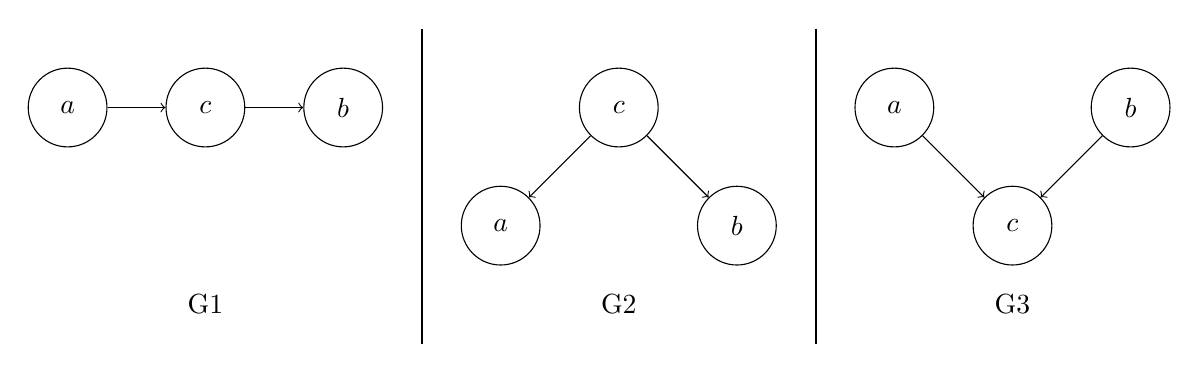
\begin{tikzpicture}
        % G1 structure
        \node[circle, draw=black, minimum size=1cm] (a1) at (0, -1.5) {$a$};
        \node[circle, draw=black, minimum size=1cm] (c1) at (1.75, -1.5) {$c$};
        \node[circle, draw=black, minimum size=1cm] (b1) at (3.5, -1.5) {$b$};
        \draw[->, black] (a1) -- (c1);
        \draw[->, black] (c1) -- (b1);
        \node at (1.75, -4) {G1};
    
        % Vertical bar between G1 and G2
        \draw[thick] (4.5, -0.5) -- (4.5, -4.5);
    
        % G2 Common Cause structure
        \node[circle, draw=black, minimum size=1cm] (c2) at (7, -1.5) {$c$};
        \node[circle, draw=black, minimum size=1cm] (a2) at (5.5, -3) {$a$};
        \node[circle, draw=black, minimum size=1cm] (b2) at (8.5, -3) {$b$};
        \draw[->, black] (c2) -- (a2);
        \draw[->, black] (c2) -- (b2);
        \node at (7, -4) {G2};
    
        % Vertical bar between G2 and G3
        \draw[thick] (9.5, -0.5) -- (9.5, -4.5);
    
        % G3 Common Effect structure
        \node[circle, draw=black, minimum size=1cm] (c3) at (12, -3) {$c$};
        \node[circle, draw=black, minimum size=1cm] (a3) at (10.5, -1.5) {$a$};
        \node[circle, draw=black, minimum size=1cm] (b3) at (13.5, -1.5) {$b$};
        \draw[->, black] (a3) -- (c3);
        \draw[->, black] (b3) -- (c3);
        \node at (12, -4) {G3};
    \end{tikzpicture}
\end{center}
请将每个情境与最合适的图模型进行匹配。(5 points)
\begin{enumerate}[(i)]
        \item 
        一个家庭的旅行决定 (\(c\)) 会受到 父母的工作安排 (\(a\)) 孩子的学校假期 (\(b\))的影响。

        \textbf{\large 解:}
        \vspace{3em}
        
        \item 
        破纪录的大雪 (\(c\))  会同时刺激 滑雪度假村的预订量 (\(a\)) 和 冬季服装的需求 (\(b\))。

        \textbf{\large 解:}
        \vspace{3em}

        \item 
        个人的锻炼习惯 (\(a\)) 会影响 自身的能量水平 (\(c\)),进而影响 工作效率 (\(b\))。

        \textbf{\large 解:}
        \vspace{3em}

        \item 
        一个地区的气候 (\(a\)) 决定了 生长的植被类型 (\(c\)),而植被类型又会影响 野生动物的数量 (\(b\))。

        \textbf{\large 解:}
        \vspace{3em}

        \item 
        一个国家的经济稳定性 (\(c\)) 会影响 就业率 (\(a\)) 和 消费者的消费习惯 (\(b\))。

        \textbf{\large 解:}
        \vspace{3em}
        
        \item 
        餐厅的受欢迎程度 (\(c\)) 取决于 食品质量 (\(a\)) 和 社交媒体的曝光度 (\(b\))。
        
        \textbf{\large 解:}
        \vspace{3em}

    \end{enumerate}




4. 考虑以下有向图,其中所有变量均为未观测变量。 (5 points)

    \begin{figure}[h]
        \centering
        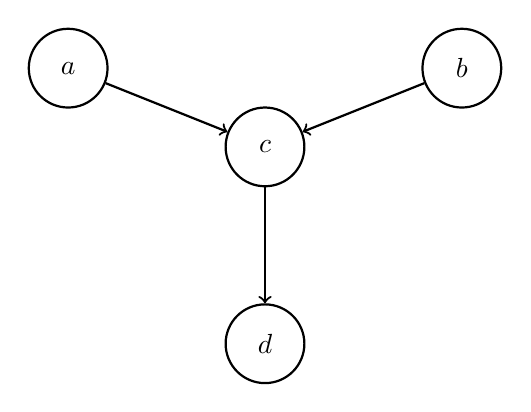
\begin{tikzpicture}
            \node[circle, draw=black, thick, minimum size=1cm] (a) at (-1.5, 2) {\(a\)};
            \node[circle, draw=black, thick, minimum size=1cm] (b) at (3.5, 2) {\(b\)};
            \node[circle, draw=black, thick, minimum size=1cm] (c) at (1, 1) {\(c\)};
            \node[circle, draw=black, thick, minimum size=1cm] (d) at (1, -1.5) {\(d\)};
            \draw[->, thick, black] (a) -- (c);
            \draw[->, thick, black] (b) -- (c);
            \draw[->, thick, black] (c) -- (d);
        \end{tikzpicture}
    \end{figure}

    \begin{enumerate}[(i)]
        \item 

        在给定的图中,如何将联合分布 $p(a, b, c, d)$ 表示为边际分布和条件分布的组合?
        
        \textbf{\large 解:}
        \vspace{3em}

        \item 

        假设 $a, b, c, d$ 是二元随机变量,求建模该联合分布所需的最小参数个数。
        
        \textbf{\large 解:}
        \vspace{3em}

        \item 
        
        证明 $a$ 和 $b$ 是相互独立的,即 \(a \perp\!\!\!\perp b\)。
        
        \textbf{\large 解:}
        \vspace{3em}


        \item 
        假设对于图中任意节点 $x$ , 都有 $p(x \mid \text{pa}(x)) \neq p(x)$, 其中 $\text{pa}(\cdot)$ 表示节点 $x$ 的父节点集合。
        证明当观测到 $d$ 时, $a$ 和 $b$ 不再相互独立, 即 \(a \not\perp\!\!\!\perp b \mid d\). 
        
        \textbf{\large 解:}
        \vspace{3em}

    \end{enumerate}

\newpage
\section*{五. (20 points) 强化学习}

在本问题中,你将思考如何通过在马尔可夫决策过程(MDP)中连续做决策来最大化奖励,并深入了解贝尔曼方程——解决和理解MDP的核心方程。

考虑经典的网格世界MDP,其中智能体从单元格 (1, 1) 开始,并在环境中导航。在这个世界中,智能体每个格子里可以采取四个动作:上、下、左、右。格子用 (水平,垂直) 来索引;也就是说,单元格 (4, 1) 位于右下角。世界的转移概率如下:如果智能体采取一个动作,它将以 0.8 的概率移动到动作的方向所在的格子,并以 0.1 的概率滑到动作的相对右或左的方向。如果动作(或滑动方向)指向一个没有可通过的格子(即边界或 (2, 2) 格子的墙壁),那么该动作将保持智能体处于当前格子。例如,如果智能体在 (3, 1) 位置,并采取向上的动作,它将以 0.8 的概率移动到 (3, 2),以 0.1 的概率移动到 (2, 1),以 0.1 的概率移动到 (4, 1)。如果智能体在 (1, 3) 位置并采取右移动作,它将以 0.8 的概率移动到 (2, 3),以 0.1 的概率移动到 (1, 2),以 0.1 的概率停留在 (1, 3)。当智能体到达定义的奖励状态时(在 (4, 2) 和 (4, 3) 单元格),智能体将获得相应的奖励,并且本次回合结束。

回顾计算MDP中每个状态的\textit{最优价值}, $V^{*}(s)$的贝尔曼方程,其中我们有一组动作$A$,一组状态$S$,每个状态的奖励值$R(s)$,我们的世界的转移动态$P(s' | s, a)$,以及折扣因子$\gamma$:
\begin{align*}
V^{*}(s) = R(s) + \gamma \max_{a \in A} \sum_{s' \in S} P(s' | s, a) V^{*}(s')
\end{align*}
最后,我们将策略表示为$\pi(s) = a$其中策略$\pi$指定了在给定状态下采取的行动。

\begin{enumerate}[(a)]
\item 
考虑一个智能体从单元格 (1, 1) 开始,在第 1 步和第 2 步分别采取向上和向上的动作。计算在每个时间步内,根据这一动作序列,智能体可以到达哪些单元格,以及到达这些单元格的概率。(6 points)

        
\textbf{\large 解:}
\vspace{3em}



\item
考虑当前没有奖励值的所有状态的奖励函数 $R(s)$(即除了 (4, 2) 和 (4, 3) 以外的每个单元格)。 定义在以下奖励值下,智能体的最优策略: (i.) $R(s) = 0$, (ii.) $R(s) = -2.0$, and (iii.) $R(s) = 1.0$. 你可以假设折扣因子接近 1,例如 0.9999。画出网格世界并标出在每个状态下应采取的动作可能会对你有所帮助(记住,策略是在 MDP 中对所有状态进行定义的!)(7 points)

\emph{注意}: 你不需要算法上计算最优策略。你必须列出每种情况的完整策略,但只需要提供直观的理由。
        
\textbf{\large 解:}
\vspace{3em}



\item
有时,MDP 的奖励函数形式为 $R(s, a)$ 它依赖于所采取的动作,或者奖励函数形式为 $R(s, a, s')$ ,它还依赖于结果状态。写出这两种形式的最优价值函数的贝尔曼方程。(7 points)
        
\textbf{\large 解:}
\vspace{3em}



\end{enumerate}

\end{document}
